\documentclass{beamer}

\usepackage{comment}
\usepackage{color}

\title{An Overview of the PFLOTRAN Input Deck}
\author{Glenn Hammond}
\date{\today}

\begin{document}

\frame{\titlepage}

\begin{comment}
\begin{frame}
%Freaking manual table of contents since beamer is stupid!!!!
\footnotesize
\begin{itemize}
\item[] {\color{blue}Syntax}
\item[] {\color{blue}Control Cards}
\begin{itemize}
\item[] SIMULATION
\end{itemize}
\item[] {\color{blue}Required Cards}
\begin{itemize}
\item[] GRID
\item[] REGION
\item[] MATERIAL\_PROPERTY
\item[] STRATA
\item[] TIME
\item[] INITIAL\_CONDITION
\end{itemize}
\item[] {\color{blue}Required Cards for Flow}
\begin{itemize}
\item[] FLOW\_CONDITION
\end{itemize}
\item[] {\color{blue}Required Cards for Reactive Transport}
\begin{itemize}
\item[] CHEMISTRY
\item[] TRANSPORT\_CONDITION
\item[] CONSTRAINT
\end{itemize}
\item[] {\color{blue}Optional Cards}
\begin{itemize}
\item[] OUTPUT
\item[] FLUID\_PROPERTY
\end{itemize}
\end{itemize}
\end{frame}
\end{comment}

\section{Syntax}
\subsection{Syntax}

\begin{frame}[fragile,containsverbatim]\frametitle{Syntax}

The PFLOTRAN input deck is defined using keywords or cards that are associated with data.  The file is designed with modularity in mind and the cards need not be in any particular order.  Many cards open a section or block that provides additional cards and is terminated by an ``END'' or ``/''.  For example:

\begin{semiverbatim}
CARD1
  CARD2 value value
  CARD3
    CARD4 value
    CARD5 value
  /
END
\end{semiverbatim}

\end{frame}

\begin{frame}[fragile]\frametitle{Syntax: Commenting}
Several options exist for commenting out lines or sections of the input file:
\begin{itemize}
\item The hash (\#) or exclamation point (!) behave similar to Fortran or shell scripts.  Everything on a line after the comment character is ignored.
\item The SKIP/NOSKIP cards may be used to comment out a large number of lines.  SKIP/NOSKIP may be used in a nested manner.  
\end{itemize}

\end{frame}

\begin{frame}[containsverbatim]\frametitle{Syntax: Commenting Example}

\begin{semiverbatim}
CARD0
SKIP
CARD1
  ! comment on CARD2
  CARD2 value1 value2
  CARD3
  !  CARD4 value3 
    CARD5 value4 # comment explaining value3
  /
  CARD6 value5 ! comment explaining value5
#  CARD7 value6
  CARD7 value7
END
NOSKIP
CARD8
\end{semiverbatim}

\end{frame}


\section{File Layout}
\subsection{Layout}

\begin{frame}[fragile,containsverbatim]\frametitle{Layout}

\begin{semiverbatim}
  SIMULATION
    # declares the process models used.
  END

  SUBSURFACE
    # defines the flow and transport process models
  END
  
  PM_BLOCK(s)
    # defines other process models
  END

\end{semiverbatim}

\end{frame}

\begin{frame}[fragile,containsverbatim]\frametitle{SUBSURFACE Layout (Minimal)}

\begin{semiverbatim}
  SUBSURFACE
    GRID               # discretization
    MATERIAL_PROPERTY  # material properties
    OUTPUT             # screen/file output
    TIME               # final time, time stepping, etc
    REGION             # regions in domain
    FLOW_CONDITION     # state variables
    INITIAL_CONDITION  # couple FLOW_CONDITION and REGION
    BOUNDARY_CONDITION # couple FLOW_CONDITION and REGION
    STRATA             # couple MATERIAL_PROPERTY and
  END                  #   REGION
\end{semiverbatim}

\end{frame}

\begin{frame}[fragile,containsverbatim]\frametitle{Coupling REGIONs to Properties and States}

\begin{semiverbatim}
  INITIAL_CONDITION
    FLOW_CONDITION pressure
    REGION source_zone
  END
  
  BOUNDARY_CONDITION inlet
    FLOW_CONDITION injection
    REGION west_face
  END
  
  STRATA
    MATERIAL soil
    REGION source_zone
  END
\end{semiverbatim}

\end{frame}

%-----------------------------------------------------------------------------
\begin{frame}[fragile,containsverbatim]\frametitle{}
\small
\begin{semiverbatim}
PFLOTRAN_DIR/shortcourse/exercises/1D_variably_saturated_flow
\end{semiverbatim}
\end{frame}

%-----------------------------------------------------------------------------
\section{Control Cards}

\subsection{SIMULATION}

\begin{frame}[fragile,containsverbatim]\frametitle{SIMULATION}

\begin{itemize}
\item[] \textbf{Purpose:} Defines 
\begin{itemize}
  \item Type of simulation
  \item Process models required
  \item Process model specific options
  \item Checkpoint/restart
\end{itemize}
\begin{comment}
\item[] \textbf{Example uses:}
\begin{itemize}
  \item 
\end{itemize}
\end{comment}
\item[] \textbf{Key sub-cards:}
\begin{itemize}
\item[] \verb|SIMULATION_TYPE|
\item[] \verb|  SUBSURFACE|
\item[] \verb|  GEOMECHANICS_SUBSURFACE|
\item[] \verb|  ...|
\item[] \verb|PROCESS_MODELS|
\item[] \verb|  SUBSURFACE_FLOW|
\item[] \verb|  SUBSURFACE_TRANSPORT|
\item[] \verb|  UFD_DECAY|
\item[] \verb|  ...|
\item[] \verb|CHECKPOINT|
\item[] \verb|RESTART|
\end{itemize}
\end{itemize}

\end{frame}

%-----------------------------------------------------------------------------
\begin{frame}[fragile]\frametitle{SIMULATION Example: Flow and Transport}

\begin{semiverbatim}
SIMULATION
  SIMULATION_TYPE SUBSURFACE
  PROCESS_MODELS
    SUBSURFACE_FLOW flow
      MODE RICHARDS
    /
    SUBSURFACE_TRANSPORT transport
      GLOBAL_IMPLICIT
    /
  /
END
\end{semiverbatim}

\end{frame}

%-----------------------------------------------------------------------------
\begin{frame}[fragile]\frametitle{SIMULATION Example: Multiphase Flow}

\begin{semiverbatim}
SIMULATION
  SIMULATION_TYPE SUBSURFACE
  PROCESS_MODELS
    SUBSURFACE_FLOW flow
      MODE GENERAL
      OPTIONS
        ANALYTICAL_JACOBIAN
        ARITHMETIC_GAS_DIFFUSIVE_DENSITY
      /
    /
  /
END
\end{semiverbatim}

\end{frame}

%-----------------------------------------------------------------------------
\begin{frame}[fragile]\frametitle{SIMULATION Example: With Checkpointing}
\begin{semiverbatim}
SIMULATION
  SIMULATION_TYPE SUBSURFACE
  PROCESS_MODELS
    SUBSURFACE_FLOW flow
      MODE TH
    /
  /
  CHECKPOINT
    PERIODIC TIMESTEP 10
    PERIODIC TIME y 100.
    TIMES y 137.
    FORMAT HDF5
  /
END
\end{semiverbatim}

\end{frame}


%-----------------------------------------------------------------------------
\section{Required Cards}

\subsection{GRID}

\begin{frame}[fragile,containsverbatim]\frametitle{GRID}

\begin{itemize}
\item[] \textbf{Purpose:} Defines the physically discretized domain
\item[] \textbf{Example uses:}
\begin{itemize}
  \item Type of discretization [structured, unstructured]
  \item Extent of domain
  \item Grid resolution
  \item Specifying direction of gravity vector
\end{itemize}
\item[] \textbf{Key sub-cards:}
\begin{itemize}
  \item[] \verb|TYPE|
  \item[] \verb|  STRUCTURED|
  \item[] \verb|  UNSTRUCTURED|
  \item[] \verb|  UNSTRUCTURED_EXPLICIT|
  \item[] \verb|ORIGIN|
  \item[] \verb|BOUNDS|
  \item[] \verb|NXYZ|
  \item[] \verb|DXYZ|
\end{itemize}
\end{itemize}

\end{frame}

%-----------------------------------------------------------------------------
\begin{frame}[fragile]\frametitle{GRID Example: Cartesian Grid with BOUNDS}

\begin{semiverbatim}
GRID
  TYPE STRUCTURED
  NXYZ 16 16 16
  BOUNDS
    0.d0 0.d0 0.d0
    16.d0 16.d0 16.d0
  /
END
\end{semiverbatim}

\end{frame}

%-----------------------------------------------------------------------------
\begin{frame}[fragile]\frametitle{GRID Example: Cartesian Grid with DXYZ}

\begin{semiverbatim}
GRID
  TYPE STRUCTURED
  ORIGIN 0.d0 0.d0 0.d0
  NXYZ 5 4 3
  DXYZ
    10. 11. 12. 13. 14.
    13. 12. 11. 10.
    15. 20. 25.
  /
END
\end{semiverbatim}

\end{frame}

%-----------------------------------------------------------------------------
\begin{frame}[fragile]\frametitle{GRID Example: Explicit Unstructured Grid}

\begin{semiverbatim}
GRID
  TYPE UNSTRUCTURED_EXPLICIT ./mixed.uge
END
\end{semiverbatim}
\textit{mixed.uge contents}
\begin{semiverbatim}
CELLS 15
1 4.0625 4.0625 4.0625 5.20833
2 4.375 4.375 3.125 2.60417
...
15 1.25 3.75 0.3125 2.60417
CONNECTIONS 24
1 2 4.16667 4.16667 3.3333 6.25
1 3 3.75 3.75 3.75 8.8388
...
14 15 0.41667 3.75 0.41667 2.2097
\end{semiverbatim}

\end{frame}

\subsection{REGION}

\begin{frame}[fragile,containsverbatim]\frametitle{REGION}

\begin{itemize}
\item[] \textbf{Purpose:} Defines a region of the physically discretized domain
\item[] \textbf{Example uses:}
\begin{itemize}
  \item Specify a 0-3D zone
  \item Specify an individual grid cell through i,j,k indices
  \item Specify a list of grid cells
\end{itemize}
\item[] \textbf{Key sub-cards:}
\begin{itemize}
  \item[] \verb|BLOCK|
  \item[] \verb|COORDINATE|
  \item[] \verb|COORDINATES|
  \item[] \verb|FACE|
  \item[] \verb|  EAST, WEST, SOUTH, NORTH, BOTTOM, TOP|
  \item[] \verb|FILE|
  \item[] \verb|CARTESIAN_BOUNDARY|
\end{itemize}
\end{itemize}

\end{frame}

%-----------------------------------------------------------------------------
\begin{frame}[fragile]\frametitle{REGION Example: Infinite}

\begin{semiverbatim}
REGION all
  COORDINATES
    -1.d20 -1.d20 -1.d20
    1.d20 1.d20 1.d20
  /
END
\end{semiverbatim}

\end{frame}

%-----------------------------------------------------------------------------
\begin{frame}[fragile]\frametitle{REGION Example: Plane}

\begin{semiverbatim}
REGION north
  FACE NORTH
  COORDINATES
    0.d0 46.d0 0.d0
    60.d0 46.d0 60.d0
  /
END
\end{semiverbatim}

\end{frame}

%-----------------------------------------------------------------------------
\begin{frame}[fragile]\frametitle{REGION Example: Point}

\begin{semiverbatim}
REGION center_of_13
  COORDINATE 1.25d0 2.91667 1.25d0
END
\end{semiverbatim}

\end{frame}

%-----------------------------------------------------------------------------
\begin{frame}[fragile]\frametitle{REGION Example: Line}

\begin{semiverbatim}
REGION well
  BLOCK 4 4 2 3 3 3
END
\end{semiverbatim}

\end{frame}

%-----------------------------------------------------------------------------
\begin{frame}[fragile]\frametitle{REGION Example: List of cell faces in file}

\begin{semiverbatim}
REGION west
  file west_of_12.ss
END
\end{semiverbatim}

\textit{west\_of\_12.ss contents}
\begin{semiverbatim}
1
Q 24 20 19 23
\end{semiverbatim}

\end{frame}



\section{MATERIAL\_PROPERTY Card}

\begin{frame}[fragile,containsverbatim]\frametitle{MATERIAL\_PROPERTY}

\begin{itemize}
\item[] \textbf{Purpose:} Defines parameters/properties associated with subsurface soil/rock.
\item[] \textbf{Example uses:}
\begin{itemize}
  \item Assigning permeability of the soil/rock formation
  \item Assigning porosity
  \item Coupling a material type with a permeability/saturation function
\end{itemize}
\end{itemize}

\end{frame}

\begin{frame}[fragile]\frametitle{MATERIAL\_PROPERTY: Examples}

\end{frame}

\section{STRATA Card}

\begin{frame}[fragile,containsverbatim]\frametitle{STRATA}

\begin{itemize}
\item[] \textbf{Purpose:} Couples a material id with a region
\item[] \textbf{Example uses:}
\begin{itemize}
  \item Assigning a material id to a region
  \item Reading in materia IDs on a cell by cell basis
\end{itemize}
\end{itemize}

\end{frame}

\begin{frame}[fragile]\frametitle{STRATA: Examples}

\end{frame}

\section{TIME Card}

\begin{frame}[fragile,containsverbatim]\frametitle{TIME}

\begin{itemize}
\item[] \textbf{Purpose:} Specifies critical times during the simulation
\item[] \textbf{Example uses:}
\begin{itemize}
  \item Defining the final time
  \item Defining initial time step size
  \item Defining maximum time step size
\end{itemize}
\end{itemize}

\end{frame}

\begin{frame}[fragile]\frametitle{TIME: Examples}

\end{frame}

\subsection{INITIAL\_CONDITION}

\begin{frame}[fragile,containsverbatim]\frametitle{INITIAL\_CONDITION}

\begin{itemize}
\item[] \textbf{Purpose:} Ties a flow and/or transport condition state variables to a region of the physical domain as initial conditions.
\item[] \textbf{Example uses:}
\begin{itemize}
  \item Define initial pressure
  \item Define initial concentration
\end{itemize}
\item[] \textbf{Key sub-cards:}
\begin{itemize}
  \item[] \verb|FLOW_CONDITION|
  \item[] \verb|TRANSPORT_CONDITION|
  \item[] \verb|REGION|
\end{itemize}
\end{itemize}

\end{frame}

%-----------------------------------------------------------------------------
\begin{frame}[fragile]\frametitle{INITIAL\_CONDITION Example: Simple}

\begin{semiverbatim}
INITIAL_CONDITION
  FLOW_CONDITION initial
  REGION plume
END
\end{semiverbatim}

\end{frame}


%-----------------------------------------------------------------------------
\begin{frame}[fragile]\frametitle{INITIAL\_CONDITION Example: Flow and Transport}

\begin{semiverbatim}
INITIAL_CONDITION
  FLOW_CONDITION initial
  TRANSPORT_CONDITION initial
  REGION all
END
\end{semiverbatim}

\end{frame}


\section{Required Cards for Flow}
\subsection{FLOW\_CONDITION}

\begin{frame}[fragile,containsverbatim]\frametitle{FLOW\_CONDITION}

\begin{itemize}
\item[] \textbf{Purpose:} Defines parameters/conditions to be associated with flow boundary and initial conditions
\item[] \textbf{Example uses:}
\begin{itemize}
  \item Specify a constant pressures on cell faces
  \item Specify a transient fluxes through cell faces
  \item Define a hydrostatic column of water
\end{itemize}
\item[] \textbf{Key sub-cards:}
\begin{itemize}
  \item[] \verb|TYPE|
  \item[] \verb|  DIRICHLET|
  \item[] \verb|  NEUMANN|
  \item[] \verb|  RATE|
  \item[] \verb|DATUM|
  \item[] \verb|GRADIENT|
  \item[] \verb|PRESSURE|
  \item[] \verb|FLUX|
  \item[] \verb|RATE|
\end{itemize}
\end{itemize}

\end{frame}

%-----------------------------------------------------------------------------
\begin{frame}[fragile]\frametitle{FLOW\_CONDITION Example: Undulating River}

\begin{semiverbatim}
FLOW_CONDITION river
  TYPE
    PRESSURE HYDROSTATIC
  /
  INTERPOLATION LINEAR
  DATUM LIST
    TIME_UNITS d
    0.d0 0.d0 0.d0 34.d0
    10.d0 0.d0 0.d0 39.d0
    50.d0 0.d0 0.d0 33.d0
    100.d0 0.d0 0.d0 34.d0
  /
  PRESSURE 101325 ! Pa
END
\end{semiverbatim}

\end{frame}

%-----------------------------------------------------------------------------
\begin{frame}[fragile]\frametitle{FLOW\_CONDITION Example: Transient Rainfall}

\begin{semiverbatim}
FLOW_CONDITION recharge
  TYPE
    FLUX NEUMANN
  /
  FLUX LIST
    TIME_UNITS yr
    DATA_UNITS cm/yr
    0.d0 25.d0
    1.d0 23.d0
    2.d0 27.d0
    3.d0 22.d0
    4.d0 24.d0
    5.d0 29.d0
  /
END
\end{semiverbatim}

\end{frame}

%-----------------------------------------------------------------------------
\begin{frame}[fragile]\frametitle{FLOW\_CONDITION Example: Permeability-Weighted Injection Well}

\begin{semiverbatim}
FLOW_CONDITION injection_well
  TYPE
    RATE SCALED_VOLUMETRIC_RATE NEIGHBOR_PERM
  /
  RATE 1 m^3/hr
END
\end{semiverbatim}

\end{frame}


\section{Required Cards for Reactive Transport}
\section{CHEMISTRY Card}

\begin{frame}[fragile,containsverbatim]\frametitle{CHEMISTRY}

\begin{itemize}
\item[] \textbf{Purpose:} Defines basis species and all chemical reactions based on those species.  Also defines output options for reactive transport.
\item[] \textbf{Example uses:}
\begin{itemize}
  \item Naming chemistry components
  \item Defining geochemistry:
    \begin{itemize}
      \item Defining basis species
      \item Aqueous speciation reactions
      \item Minerals and mineral reactions
      \item Activity calculations
      \item Database name
    \end{itemize}
\end{itemize}
\end{itemize}

\end{frame}

\begin{frame}[fragile]\frametitle{CHEMISTRY: Examples}

\end{frame}

\section{TRANSPORT\_CONDITION Card}

\begin{frame}[fragile,containsverbatim]\frametitle{TRANSPORT\_CONDITION}

\begin{itemize}
\item[] \textbf{Purpose:} To specify solute concentrations to be associated with a transport boundary/initial condition or source/sink
\item[] \textbf{Example uses:}
\begin{itemize}
  \item Assigning time varying concentrations at a boundary
  \item Specifying the initial species composition of the fluid
  \item Assigning a boundary condition type (e.g. Dirichlet, Neumann, zero gradient)
\end{itemize}
\end{itemize}

\end{frame}

\begin{frame}[fragile]\frametitle{TRANSPORT\_CONDITION: Examples}

\end{frame}

\subsection{CONSTRAINT}

\begin{frame}[fragile,containsverbatim]\frametitle{CONSTRAINT}

\begin{itemize}
\item[] \textbf{Purpose:} A snapshot of chemistry
\item[] \textbf{Example uses:}
\begin{itemize}
  \item Defining aqueous chemistry
  \item Defining mineralogy
\end{itemize}
\item[] \textbf{Key sub-cards:}
\begin{itemize}
  \item[] \verb|CONCENTRATIONS|
  \item[] \verb|SURFACE_COMPLEXES|
  \item[] \verb|IMMOBILE|
  \item[] \verb|MINERALS|
\end{itemize}
\end{itemize}

\end{frame}

%-----------------------------------------------------------------------------
\begin{frame}[fragile]\frametitle{CONSTRAINT Example: Solutes}

\begin{semiverbatim}
CONSTRAINT initial
  CONCENTRATIONS
    Tracer  1.d-10 T
    Tracer2 1.d-10 T
  /
END
\end{semiverbatim}

\end{frame}

%-----------------------------------------------------------------------------
\begin{frame}[fragile]\frametitle{CONSTRAINT Example: Carbonate Chemistry}

\begin{semiverbatim}
CONSTRAINT equilibrated
  CONCENTRATIONS
    H+     1.d-8      F
    HCO3-  1.d-3      G  CO2(g)
    Ca++   5.d-4      M  Calcite
  /
  MINERALS
    Calcite 1.d-5 1.d0 m^2/m^3
  /
END
\end{semiverbatim}

\end{frame}


%-----------------------------------------------------------------------------
\section{Optional Cards}
\documentclass{beamer}

\usepackage{comment}
\usepackage{color}
\usepackage{tabbing}

\title{Types of PFLOTRAN Boundary Conditions\\ Basic}
\author{Glenn Hammond}
\date{\today}

\begin{document}

\frame{\titlepage}

%-----------------------------------------------------------------------------
\section{Flow}
\subsection{Types of Flow Conditions}

\begin{frame}[fragile,containsverbatim]\frametitle{Types of Flow Conditions}

\vspace{0.1in}
\centering
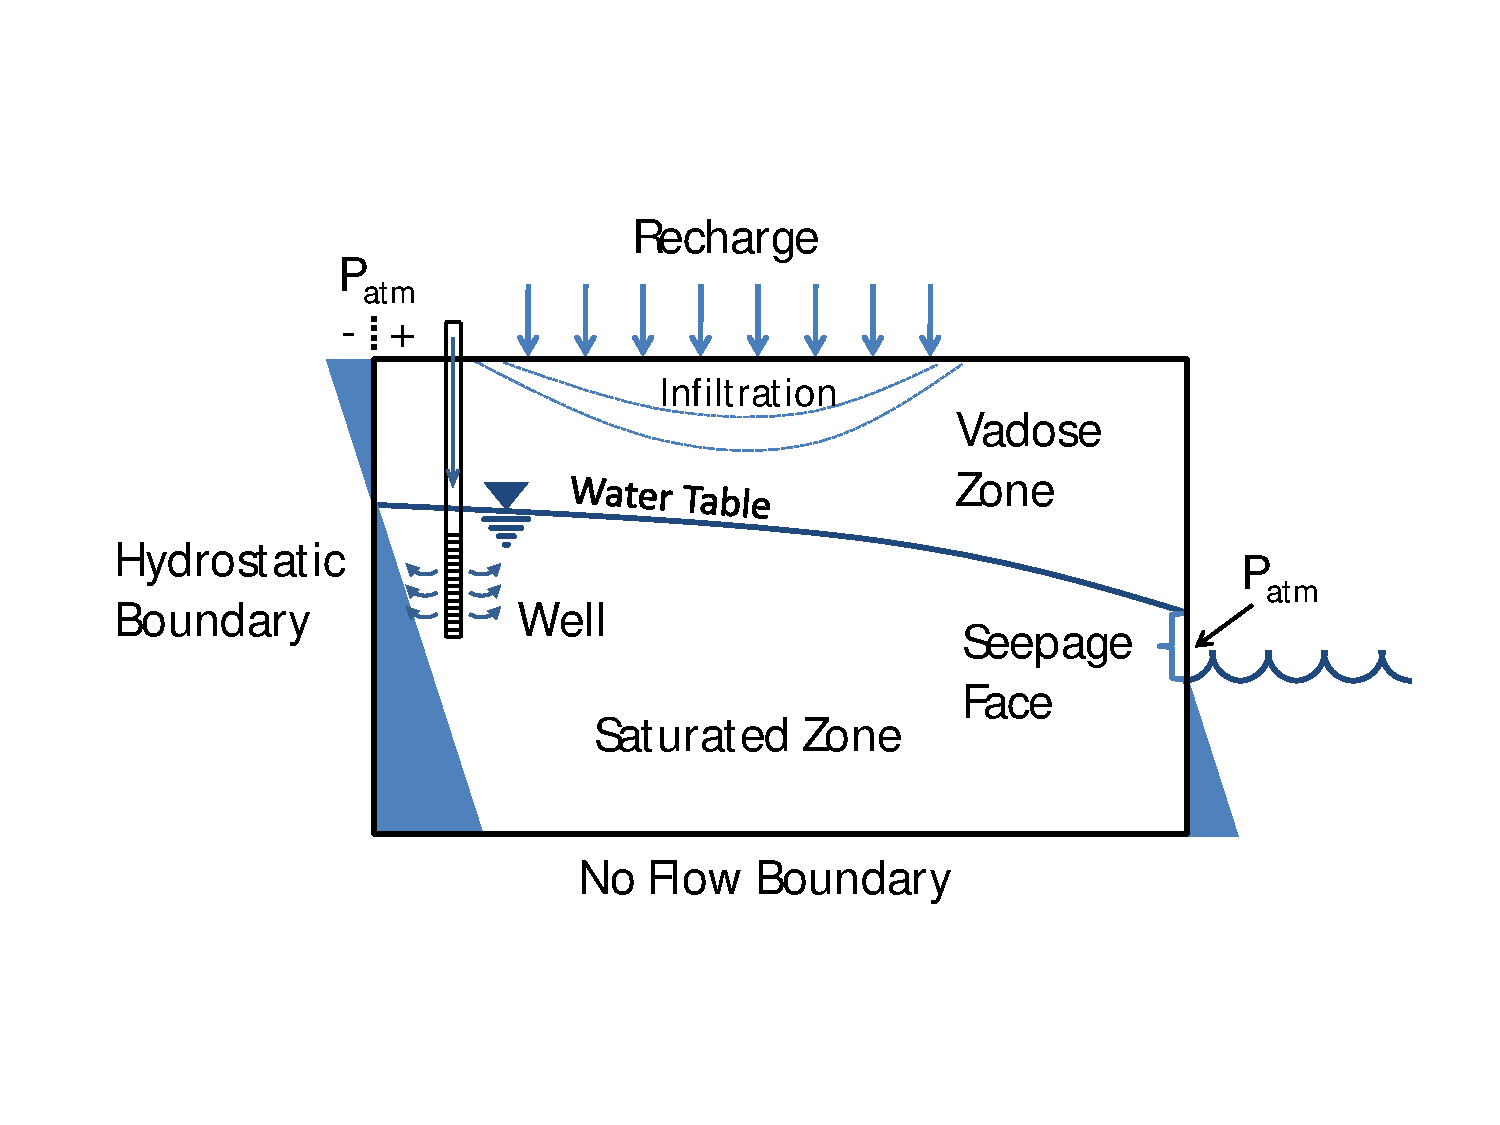
\includegraphics[width=0.9\linewidth]{./flow_bcs_with_well}
%\vspace{-0.5in}
\small 
\begin{tabbing}
\verb|DIRICHLET        |	\= Specified pressure across region\\
\verb|HYDROSTATIC|	      \> Hydrostatic pressure profile across region\\
\verb|SEEPAGE|	         	\> Hydrostatic with outflow only above water table\\
\verb|NEUMANN|			      \> Darcy flux across boundary [L/T]\\
\verb|MASS_RATE|	      	\> Mass injection/extraction rate [M/T]\\
\verb|VOLUMETRIC_RATE|	  \> Volumetric injection/extraction rate [L$^3$/T]\\
\end{tabbing}

\end{frame}


\section{Transport}
\subsection{Types of Transport Conditions}

\begin{frame}[fragile,containsverbatim]\frametitle{Types of Transport Conditions}

\vspace{0.1in}
\centering
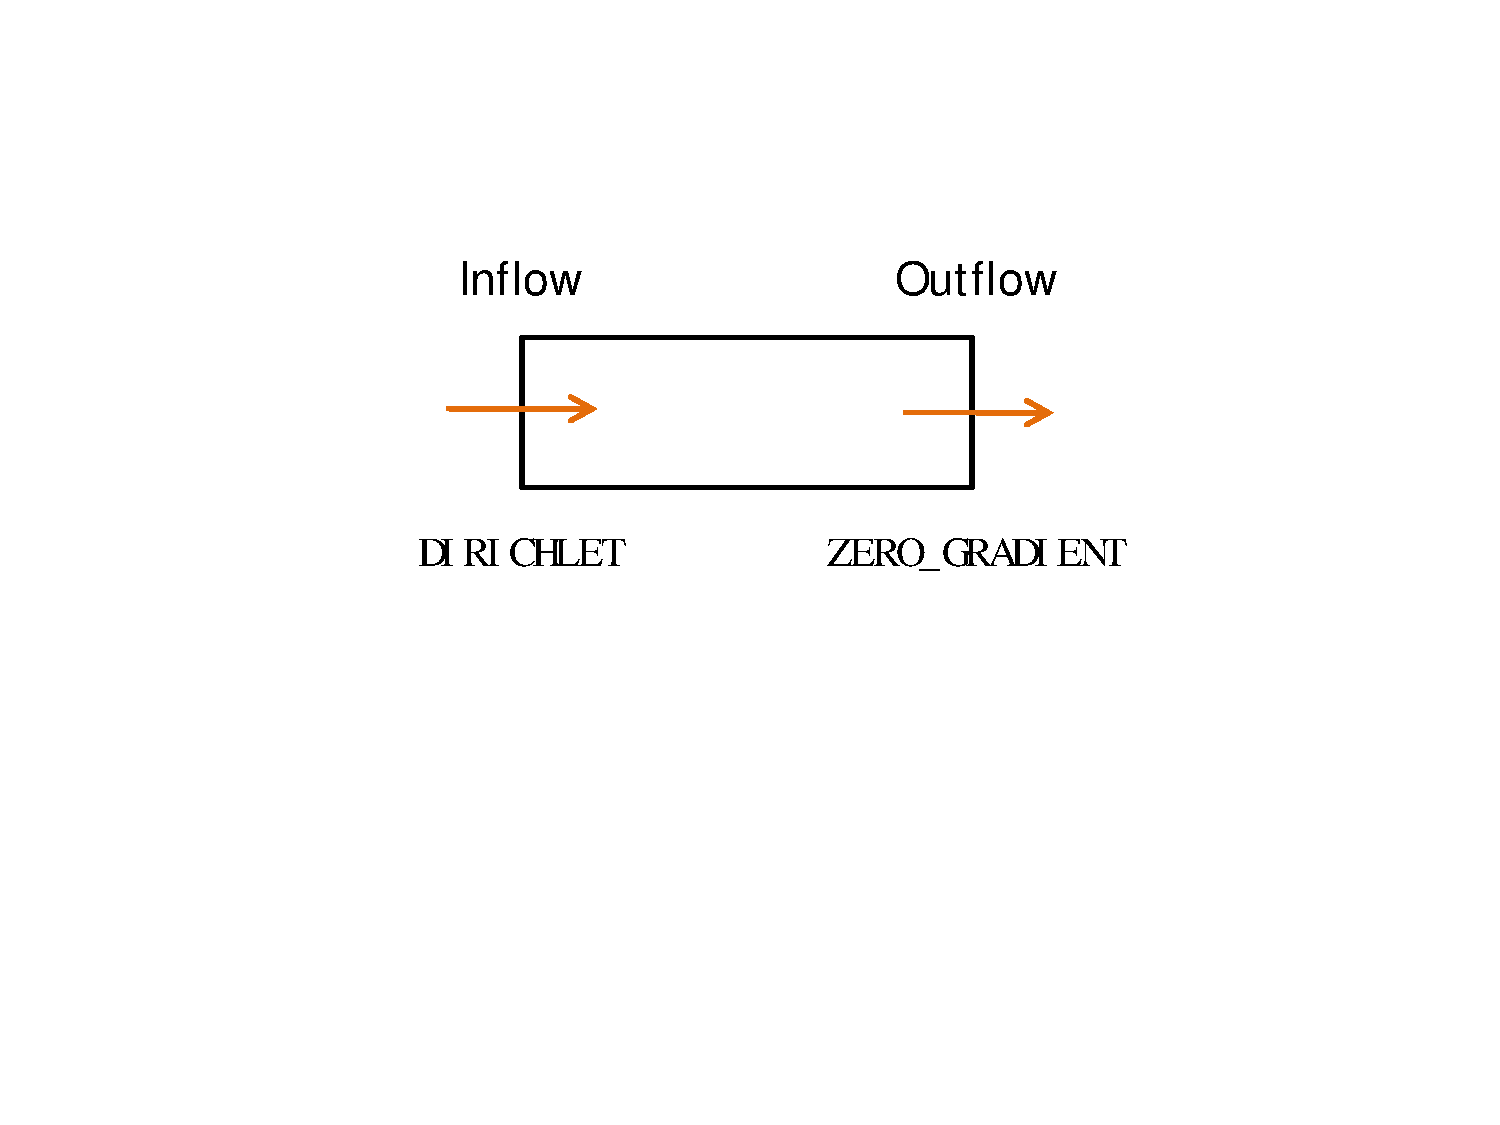
\includegraphics[width=0.5\linewidth]{./transport_bcs_unidirectional}
\vspace{0.1in}
%\hline
\vspace{0.1in}
\hspace{-6mm}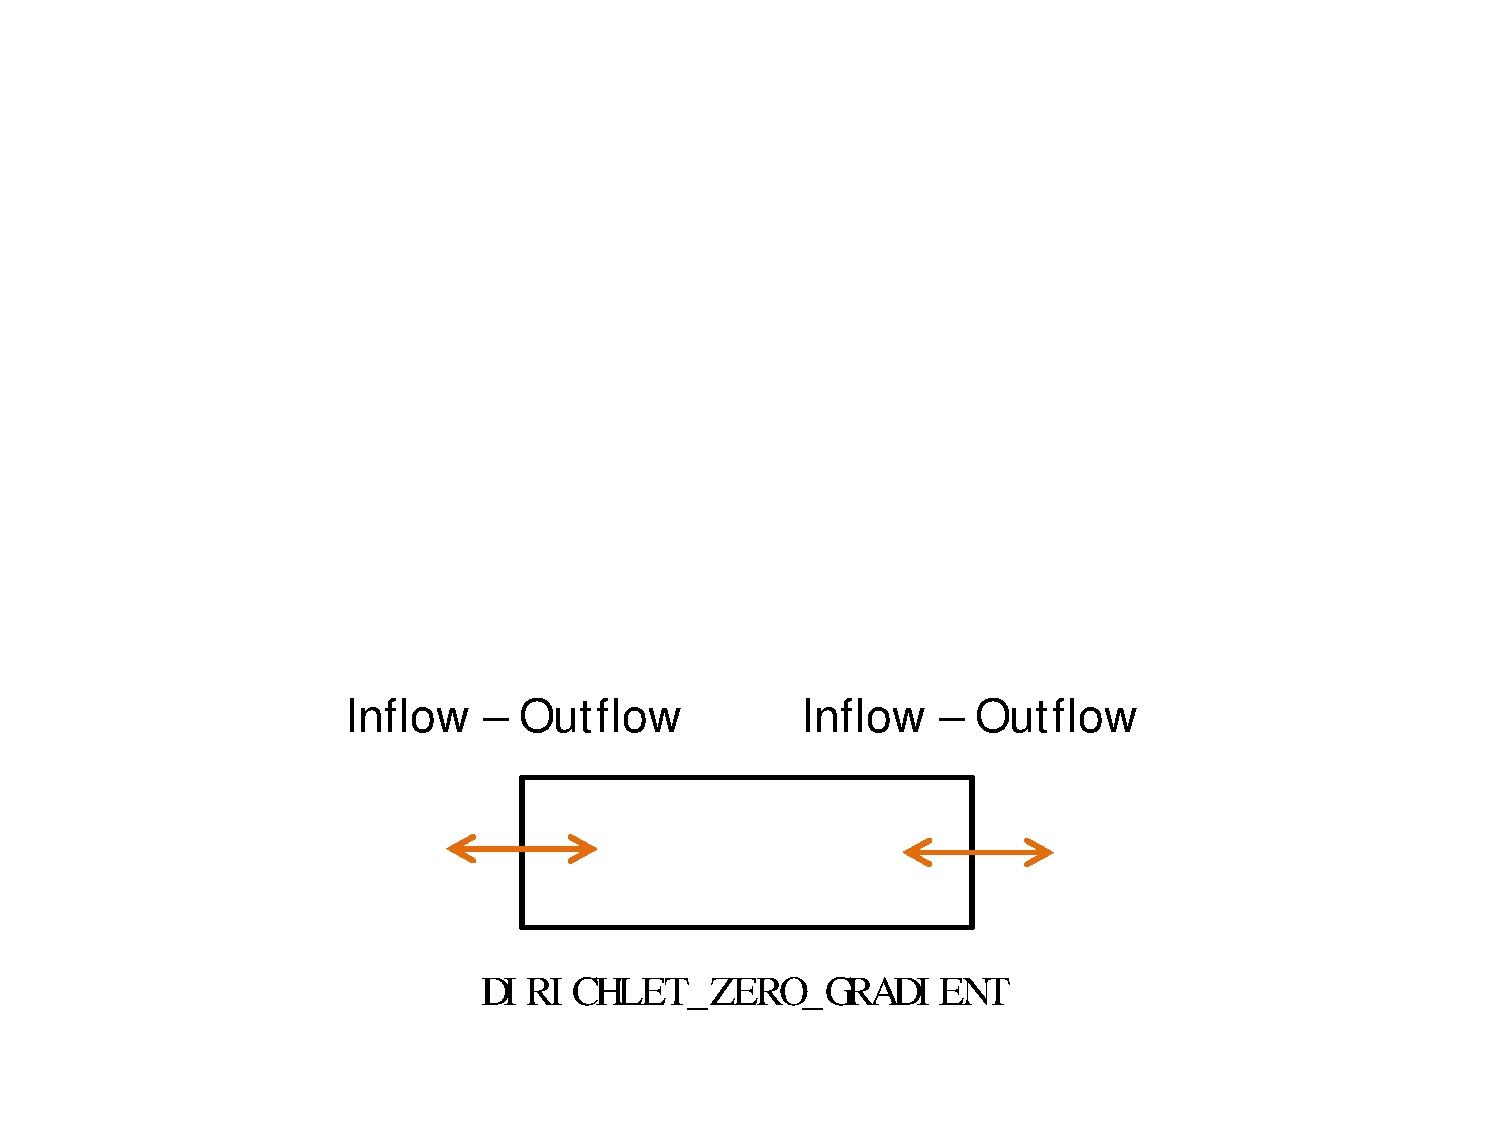
\includegraphics[width=0.58\linewidth]{./transport_bcs_bidirectional}

\begin{tabbing}
\verb|DIRICHLET                 |	\= Specified concentration\\
\verb|ZERO_GRADIENT|     	        \> Zero diffusive flux\\
\verb|DIRICHLET_ZERO_GRADIENT|		\> Hybrid for inflow - outflow
\end{tabbing}

\end{frame}




\end{document}
\section{OUTPUT Card}

\begin{frame}[fragile,containsverbatim]\frametitle{OUTPUT}

\begin{itemize}
\item[] \textbf{Purpose:} Defines output parameters such as output times, output frequency, file formats, advanced output (e.g. mass balance calculations, observation points)
\item[] \textbf{Example uses:}
\begin{itemize}
  \item Setting the output frequency to every 100 time steps
  \item Requesting output at 100.5 years
  \item Requesting both ASCII and binary HDF5 formats
  \item Differentiating between Tecplot point versus block formats
\end{itemize}
\end{itemize}

\end{frame}

\begin{frame}[fragile]\frametitle{OUTPUT: Examples}

\end{frame}

\section{FLUID\_PROPERTY Card}

\begin{frame}[fragile,containsverbatim]\frametitle{FLUID\_PROPERTY}

\begin{itemize}
\item[] \textbf{Purpose:} Define fluid properties
\item[] \textbf{Example uses:}
\begin{itemize}
  \item Assigning a coefficient of diffusion
\end{itemize}
\end{itemize}

\end{frame}

\begin{frame}[fragile]\frametitle{FLUID\_PROPERTY: Examples}

\end{frame}


\end{document}